% ============================================================================
%  第 5 章 类域论（原书 pp. 61--74）
%  译自 David Ben-Zvi, "Between Electric-Magnetic Duality and the Langlands Program"
%  Lecture notes by Jackson Van Dyke, UT Austin, Spring 2021.
% ============================================================================
\chapter{类域论}\label{ch:05}

\begin{keytakeaways}
数论（具体说是类域论）是与拓扑、物理并列的另一类对偶来源。对 数域 $F$，
理想类群 $\mathcal{C}\ell(F)=\mathrm{Pic}(\Spec\cO_{F})$ 是有限群，而（非分歧）
类域论把它与 Galois 群联系起来：$\mathcal{C}\ell(F)\simeq\Gal(F^{ur,ab}/F)$ 恰是
Hilbert 类域的自同构群。取特征便得到 Pontrjagin 对偶
$\Loc_{\GG_{m}}(\cO_{F})=\Hom(\mathcal{C}\ell(F),\C^{\times})$。在函数域情形，
$\mathrm{Pic}(C)$ 与“非分歧 Weil 群的交换化”$W_{C}^{ur,ab}$ 之间的对照（定理 2）
给出 $(\mathrm{Pic}(C))^{\vee}\simeq\Loc_{1}(C)$，即 $\mathrm{Pic}$ 上的函数与
$\Loc$ 上的函数之间的 Fourier 变换；此时 Hecke 算子 $L\mapsto L(x)$ 扮演
't Hooft 算子的角色，而 $\rho\mapsto\rho(\mathrm{Fr}_{x})$ 扮演 Wilson 算子的
角色。把 $\Spec\cO_{F}$ 看成（无向的）3-流形，这套对偶就是 Artin--Verdier
对偶。最后允许分歧：物理上挖去一个结与在结上做平凡化互为对偶；算术上温和分歧的
局部系统 $\Loc_{1}(C\setminus S)^{tame}$ 对偶于在 $S$ 上平凡化的线丛
$\mathrm{Pic}(C,S)$，而局部类域论 $\widehat{K^{\times}}\simeq\Gal^{ab}$ 说明这些
群在 $\F_{q}^{\times}$ 与 $\widehat{\Z}$ 上的商正好对应拓扑情形里看到的那些因子。
\end{keytakeaways}

拓扑与物理给了我们一类有趣的对偶陈述。数论，具体说是\term{类域论}{class field theory}
（CFT），是另一类来源。$\mathrm{Pic}$ 的拓扑（例如局部常值函数）仍将与 $\Loc$
的代数几何（例如代数函数）互换。但在这个语境中我们需要重新解释 $\mathrm{Pic}$
与 $\Loc$。

% [Tutor Note: 这里的缩写 CFT 指 class field theory（类域论），但在数学物理
% 文献中 CFT 通常指 conformal field theory（共形场论）。本书第四章讨论的是
% 拓扑场论与超对称，本章讨论的是类域论；阅读时务必按上下文区分这两个 CFT。]

设 $F/\Q$ 是数域。记 $\mathcal{C}\ell(F)$ 为\term{理想类群}{ideal class group}。
可以把它看成：
\begin{equation}\tag{5.1}
\mathcal{C}\ell(F)=\mathrm{Pic}(\Spec\cO_{F}),
\end{equation}
它由 $\Spec\cO_{F}$ 上的线丛组成，即秩 1 投射 $\cO_{F}$-模模同构。具体地说，
类群是
\begin{equation}\tag{5.2}
\mathcal{C}\ell(F)=\text{$\cO_{F}$ 的分式理想}\big/\text{主理想}.
\end{equation}
注意这是一个交换群。事实证明 $\mathcal{C}\ell(F)$ 还是有限群，其阶是 $F$ 的一个
重要不变量，称为\term{类数}{class number}。类域论的一般哲学是把类群与 Galois 群
联系起来。

\section{非分歧类域论}
\begin{sectionkey}
非分歧类域论把理想类群与 Galois 群的交换化等同起来：
$\mathcal{C}\ell(F)\simeq\Gal(F^{ur,ab}/F)=\Aut(\text{Hilbert 类域})$。取特征后，
$\Loc_{\GG_{m}}(\cO_{F})=\Hom(\mathcal{C}\ell(F),\C^{\times})=\mathcal{C}\ell(F)^{\vee}$，
这正是算术拓扑字典中“$\Spec\cO_{F}$ 像 3-流形”的 Poincaré 对偶，即
Artin--Verdier 对偶。
\end{sectionkey}

非分歧类域论识别出：
\begin{equation}\tag{5.3}
\C\bigl[\mathcal{C}\ell(F)\bigr]\simeq\C\bigl[\Loc_{\GG_{m}}(\cO_{F})\bigr].
\end{equation}
但我们需要明确在这个语境中 $\Loc$ 是什么。我们总可以把 $\Loc$ 想成由 $\pi_{1}$
的表示组成，也可以写成：
\begin{equation}\tag{5.4}
\pi_{1}(M)=\Aut\bigl(\widetilde{M}\bigr),
\end{equation}
其中 $\widetilde{M}$ 是 $M$ 的万有覆叠。在这个语境中我们有
\begin{equation}\tag{5.5}
\Gal(E/F)=\Aut_{F}(E),
\end{equation}
而万有覆叠的类似物是 $F$ 的\term{最大非分歧扩张}{maximal unramified extension}，
记作 $F^{ur}$。于是 $\pi_{1}$ 的类似物是
\begin{equation}\tag{5.6}
\pi_{1}^{\text{ét}}(\Spec\cO_{F})=\Gal(F^{ur}/F).
\end{equation}

% [Tutor Note: (5.3) 原文印作 “$\C[\mathcal{C}\ell(f)]$”，其中 $f$ 小写，
% 明显是 $F$ 的笔误。另外这里 $\C[-]$ 是“函数空间”的记号（更准确地说，
% 是对于有限群 $\mathcal{C}\ell(F)$ 的函数空间），与 (4.72) 中群代数的含义
% 相同；两边都是有限维的，因为 $\mathcal{C}\ell(F)$ 有限。]

\begin{figure}[htbp]
  \centering
  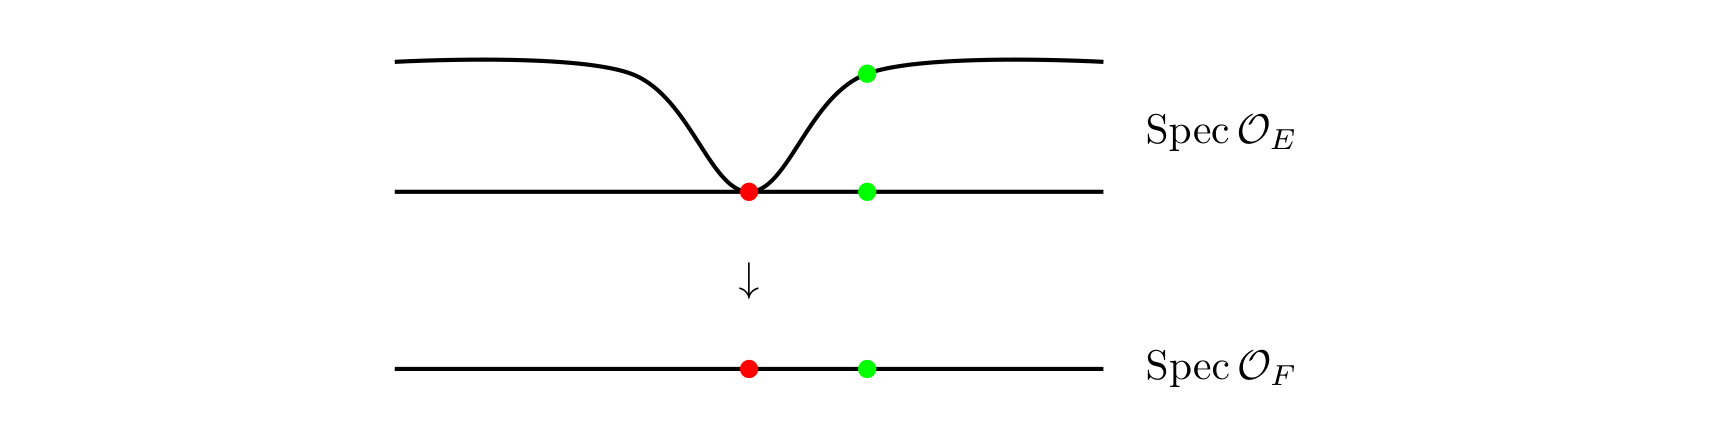
\includegraphics[width=0.72\textwidth]{figure5-1.png}
  \caption{一个在红点处分歧（左）、在绿点处非分歧（右）的扩张。（原文 p.~62，Figure 5.1）}
  \label{fig:5-1}
\end{figure}

% 说明：figure5-1.png 已包含整幅原图（上层 Spec O_E、中间竖直箭头、下层 Spec O_F）；
% figures/inline/p062_d1.png 只是同一图上半部分的放大裁剪，故此处不再重复插入。

我们取 $F^{ur}$，是因为我们要考虑 $\Spec\cO_{F}$ 的覆叠，而不是 $F$ 本身的
覆叠。我们说 $E/F$ 在素理想 $\mathfrak{p}$ 处\term{非分歧}{unramified}，如果
\begin{equation}\tag{5.7}
\cO_{E}\otimes_{\cO_{F}}\cO_{F}/\mathfrak{p}\;(=\cO_{E}/\mathfrak{p})
\end{equation}
是域的乘积，即它没有幂零元。想法是：有 $\Spec\cO_{E}$ 生活在 $\Spec\cO_{F}$
之上，而我们不希望出现图 \ref{fig:5-1} 那样的分叉。也就是说，如果看基中一点的
原像，我们希望得到域的乘积。如果出现幂零，那就说明该点处有某种有趣的几何，
我们现在想避开它。任意扩张在分歧点之外仍将扮演覆叠空间的作用。
$E/F$ 在 $\infty$ 处\term{非分歧}{unramified}，如果它们之间没有 $\C/\R$ 型的
扩张。例如 $F$ 是全虚的。想法是：与 $\R$ 做张量积对应于限制到无穷远处的邻域。
但这只是一堆 $\R$ 与 $\C$ 的拷贝：
\begin{equation}\tag{5.8}
\cO_{F}\otimes_{\Q}\R=\R^{r}\times\C^{s},
\end{equation}
然后我们要求从 $F$ 到 $E$ 的过程绝不涉及从 $\R$ 到 $\C$ 的扩张。

现在基础打好了，我们可以陈述：非分歧类域论告诉我们
\begin{equation}\tag{5.9}
\mathcal{C}\ell\simeq\Gal\bigl(F^{ur,ab}/F\bigr)=\Aut(\text{Hilbert 类域}),
\end{equation}
其中 \term{Hilbert 类域}{Hilbert class field} 是 $F$ 的最大交换扩张，且处处非分歧。

为了与此前所见的东西建立联系，我们应当研究这个 Galois 群的特征。也就是说，
一边我们有 $\mathrm{Pic}$ 的类似物 $\mathcal{C}\ell$，另一边 $\Loc$ 的类似物是：
\begin{equation}\tag{5.10}
\Hom\bigl(\Gal(F^{ur}/F),\C^{\times}\bigr).
\end{equation}
要点是：映入交换群的同态会分解到交换商上：
\begin{equation}\tag{5.11}
\Hom\bigl(\Gal(F^{ur}/F),\C^{\times}\bigr)
=\Hom\bigl(\Gal(F^{ur,ab}/F),\C^{\times}\bigr).
\end{equation}

\begin{srcrem}{20}
$\Gal(F^{ur}/F)$ 是 $\pi_{1}(\Spec\cO_{F})$ 的类似物，而
$\Gal(F^{ur,ab}/F)$ 是 $H_{1}(\Spec\cO_{F})$ 的类似物。所以这两个 $\Hom$ 空间
相等，类比于从 $\pi_{1}(\Spec\cO_{F})$ 出发的态射分解过它的交换化
$H_{1}(\Spec\cO_{F})$。
\end{srcrem}

% [Tutor Note: 这里“类似物”的层次要对齐：拓扑侧是
% $\pi_{1}\to H_{1}=\pi_{1}^{ab}$，算术侧是
% $\Gal(F^{ur}/F)\to\Gal(F^{ur,ab}/F)$。注意 (5.9) 已经用了交换化，
% 所以 (5.10)--(5.11) 的分解正是“特征只看见交换商”这一事实的特例；
% 反过来，这也说明单靠特征无法恢复非交换的 $\Gal(F^{ur}/F)$。]

于是由 (5.9)，这就是类群的 Pontrjagin 对偶：
\begin{align}
\Loc_{\GG_{m}}(\cO_{F})&=\Hom\bigl(\Gal(F^{ur}/F),\C^{\times}\bigr)\tag{5.12}\\
&=\Hom\bigl(\Gal(F^{ur,ab}/F),\C^{\times}\bigr)\tag{5.13}\\
&=\Hom\bigl(\mathcal{C}\ell(F),\C^{\times}\bigr)\tag{5.14}\\
&=\mathcal{C}\ell(F)^{\vee}.\tag{5.15}
\end{align}

\begin{srcrem}{21}
Artin--Verdier 对偶是 $\Spec\cO_{F}$ 上 Poincaré 对偶的类似物。这是我们建立
算术拓扑字典的基础，该字典说数域（或更确切地说 $\Spec\cO_{F}$）类比于
一个 3-流形。回忆对 3-流形而言 $\mathrm{Pic}$ 与 $\Loc$ 之间的对偶就是
Poincaré 对偶，而这个类域论的重述正是 Artin--Verdier 对偶的陈述。但
Artin--Verdier 对偶的建立依赖于类域论，所以这并不是用来证明类域论的方向。
\end{srcrem}

\begin{srcrem}{22}
算术拓扑字典告诉我们 $\Spec\cO_{F}$ 对应于一个 3-流形。结果表明它是一个
\emph{无向}的 3-流形。也就是说，对偶化对象不是常值对象。这种定向的缺失类比于
以下差别：
\begin{itemize}
\item $\Z/n$ 与单位根 $\mu_{n}$，
\item $\Q/\Z$ 与 $\mu_{\infty}$，
\item $\C^{\times}$ 与 $\GG_{m}$，等等。
\end{itemize}
结果表明，对偶化对象不是 $\Z$，而是 Tate 扭 $\Z(1)$（$\mu_{n}$ 相对于
$\Z/p\Z$ 的代数闭包）。在 Gauss 定律中，或者在计算线丛的 Chern 类时，
我们遇到过一些 $2\pi i$ 因子。它们正是由这一现象来解释的。
\end{srcrem}

% [Tutor Note: $\Z(1)=\varprojlim\mu_{n}$ 是 Tate 模，其“取向”相当于选取
% 一个相容的单位根系统；$\R$ 上的对应物是 $2\pi i\Z$。这就是为什么 (4.19)
% 中的 $b_{\Sigma}=\frac{1}{2\pi i}\int F$ 与 (5.80) 的 Lefschetz 对偶里
% 都会出现 $2\pi i$：算术侧用 $\Z(1)$ 代替 $\Z$，等价于在拓扑侧把常值系数
% 换成带 twist 的系数。原文说“$\mu_n$ with respect to the algebraic closure
% of $\Z/p\Z$”，准确说法应是“相对于 $\Spec\F_{p}$ 的代数闭包的 $p$-进 Tate 模”。]

把 $\Gal^{ur}$ 的特征与 $\mathcal{C}\ell^{\vee}_{F}$ 等同起来的结论是：我们得到
一个 Fourier 变换
\begin{equation}\tag{5.16}
\C[\mathcal{C}\ell_{F}]\simeq\C\bigl[\Loc_{1}(\Spec\cO_{F})\bigr],
\end{equation}
其中 $\Loc_{1}$ 定义为 $\Gal^{ur}$ 的特征。

\begin{flushright}\small 第 9 讲；2021 年 2 月 23 日\end{flushright}

\begin{srcex}{28}
若 $F=\Q$，则两边都是平凡的。
\end{srcex}

\section{函数域}
\begin{sectionkey}
在函数域情形，$\mathrm{Pic}(C)$（线丛模同构）与“非分歧 Weil 群的交换化”
$W_{C}^{ur,ab}$ 满足同样的三条性质：都满射到 $\Z$、都交换、且对每个 $k$-点有
截面。定理 2 断言它们在投射有限完备化上同构；取特征后得到
$(\mathrm{Pic}(C))^{\vee}\simeq\Loc_{1}(C)$，从而有 $\mathrm{Pic}$ 与 $\Loc$
之间的 Fourier 变换，Hecke 算子对应于 't Hooft 算子，Frobenius 的特征值对应于
Wilson 算子。
\end{sectionkey}

设 $C$ 是某个域 $k$ 上的光滑射影曲线。对它我们可以附着上\term{函数域}{function field}
$F=k(C)$，即 $C$ 上有理函数构成的域。我们也可以考虑 \term{Picard 群}{Picard group}
$\mathrm{Pic}(C)$，其 $k$-点由下式给出：
\begin{align}
\mathrm{Pic}(C)(k)&=\{\text{$C$ 上的线丛}\}/\sim\tag{5.17}\\
&=\{\text{局部自由秩 1 的 $\cO_{C}$-模}\}\tag{5.18}\\
&=\{\text{除子}\}/\{\text{主除子}\}\tag{5.19}\\
&=H^{1}(C,\cO^{\times})\tag{5.20}
\end{align}
最后一行我们用转移函数（即 Čech 上链）来刻画线丛。每个线丛都有一个\term{次数}{degree}，
它是整数。如果把线丛想成由和式 $\sum_{x\in C}n_{x}x$ 给出，那么这具体地由映射
\begin{equation}\tag{5.21}
\begin{array}{ccc}
\mathrm{Pic} & \xrightarrow{\ \deg\ } & \Z\\[2pt]
\sum_{x\in C}n_{x}x & \longmapsto & \sum n_{x}
\end{array}
\end{equation}
给出，它满射，其核为
\begin{equation}\tag{5.22}
0\to \mathrm{Jac}\to\mathrm{Pic}\to\Z\to 0,
\end{equation}
其中 $\mathrm{Jac}$ 是\term{Jacobi 簇}{Jacobian}，即次数为 0 的线丛。对任意
选定的 $x\in C$，我们都得到一份 $\Z x\hookrightarrow\mathrm{Pic}$，即这个扩张是
可裂的，且对曲线上每个点都有一个截面。

若 $k=\F_{q}$ 有限，这与我们从 $C$ 的（平展）基本群看到的东西类似。它不以 $\Z$
为商，而是以\term{投射有限完备化}{profinite completion}\footnote{回忆投射有限
完备化是所有有限商的逆向极限。} $\widehat{\Z}$ 为商：
\begin{equation}\tag{5.23}
\pi_{1}^{\text{ét}}(C)\twoheadrightarrow\widehat{\Z}=\pi_{1}^{\text{ét}}(\Spec k).
\end{equation}
想法是：曲线 $C$ 生活在 $\Spec k$ 之上，于是对 $\Spec k$ 的一个覆叠，我们可以
把它拉回成 $C$ 的覆叠 $\widetilde{C}$。这对应于从 $C$ 的基本群到 $\Spec k$ 的
基本群的映射。这与上面的情形看起来非常相似：$\mathrm{Pic}$ 以 $\Z$ 为商，
但有两个主要区别：
\begin{enumerate}
\item $\pi_{1}^{\text{ét}}$ 不是交换的，以及
\item $\widehat{\Z}$ 不是 $\Z$。
\end{enumerate}
我们可以用两种不同方式处理。第一件可做的事是把
$\pi_{1}^{\text{ét}}=\Gal^{ur}(F)$ 换成 $C$ 的\term{非分歧 Weil 群}{unramified Weil group}，
记作 $W_{C}^{ur}$。想法是我们想让 $\Spec k$ 看起来更像 $S^{1}$，于是把
$\widehat{\Z}$ 换成 $\Z$，而 $W_{C}^{ur}$ 就是 $\Z$ 在
$\pi_{1}^{\text{ét}}$ 中的原像：
\begin{equation}\tag{5.24}
\begin{array}{ccc}
\pi_{1}^{\text{ét}} & \longrightarrow & \widehat{\Z}\\[2pt]
\uparrow & & \uparrow\\[2pt]
W_{C}^{ur} & \longrightarrow & \Z
\end{array}
\end{equation}
另一件可做的事是过渡到交换化：$W_{C}^{ur,ab}$，它以 $\Z$ 为商：
\begin{equation}\tag{5.25}
W_{C}^{ur,ab}\twoheadrightarrow\Z.
\end{equation}
对每个点 $x\in C(k)$ 这个映射也有一个截面，正如上面 $\mathrm{Pic}$ 的情形。
一个点是映射 $x\colon\Spec k\to C$，几何上这给出一个映射
\begin{equation}\tag{5.26}
\widehat{\Z}=\pi_{1}^{\text{ét}}(k)\to\pi_{1}^{\text{ét}}(C),
\end{equation}
它就是相应的截面。图景是：$\Spec k$ 是圆的类似物，而 $C$ 是纤维化于其上的
3-流形的类似物。于是 $C$ 的一个 $k$-点就是一个截面，即 $C$ 中的一个环路。
总结一下，断言是：$\mathrm{Pic}$ 与 $W_{C}^{ur,ab}$ 二者都

% [Tutor Note: (5.24) 中 $W_{C}^{ur}$ 的定义是
% $W_{C}^{ur}:=(\pi_{1}^{\text{ét}})^{-1}(\Z)\subset\pi_{1}^{\text{ét}}$，
% 其中 $\Z\subset\widehat{\Z}$ 是自然包含。这个构造的意义在于：把
% $\Gal(\overline{\F}_{q}/\F_{q})\cong\widehat{\Z}$ 换成它的稠密子群 $\Z$
% （Frobenius 生成的子群），就得到“几何基本群 + Frobenius”的半直积结构；
% 这使 Weil 群成为比 $\pi_{1}^{\text{ét}}$ 更接近拓扑基本群的对象。]

\begin{itemize}
\item 满射到 $\Z$，
\item 交换，且
\item 对每个 $x\in C(k)$ 都有截面。
\end{itemize}

我们可以不改变有限域的图景，而改为改动 $\mathrm{Pic}$。回忆 $\mathrm{Pic}$ 是
$\Z$ 被 Jacobi 簇扩张，而后者在有限域上是有限群。因此 $\mathrm{Pic}$ 的所有
“无穷部分”都来自 $\Z$。于是我们可以把 $\mathrm{Pic}$ 换成它的投射有限完备化
$\widehat{\mathrm{Pic}}$。这样我们就得到一个对象：它满射到 $\widehat{\Z}$，
并且对每个点 $x\in C$ 有截面。无论如何，定理的内容就是它们匹配。

\begin{srcthm}{2}（非分歧类域论）
存在一个映射 $\mathrm{Pic}\to\pi_{1}^{\text{ét},ab}$，它在投射有限完备化上
是同构。等价地，我们有一个同构
\begin{equation}\tag{5.27}
\mathrm{Pic}\simeq W_{C}^{ur,ab},
\end{equation}
它保持取线丛次数的运算，并保持与 $x\in C$ 相关联的截面。
\end{srcthm}

% [Tutor Note: 定理 2 的准确含义是：$\mathrm{Pic}(C)$ 与
% $\pi_{1}^{\text{ét}}(C)^{ab}$ 的投射有限完备化同构，即
% $\widehat{\mathrm{Pic}(C)}\cong\pi_{1}^{\text{ét}}(C)^{ab}$；由于
% $\mathrm{Pic}$ 已是 $\Z$ 被有限群 $\mathrm{Jac}$ 的扩张，取完备化只是把
% $\Z$ 换成 $\widehat{\Z}$。这就是为什么 (5.27) 右边写 $W_C^{ur,ab}$：
% $W_C^{ur,ab}$ 正是以 $\Z$ 为商（而非 $\widehat\Z$）的那个版本。原文的
% “isomorphism on profinite completions” 一句容易误读成“两个群本身同构”，
% 实际上只是完备化后同构。另外，本章的定理编号是 “定理 2”“定理 3”，与章节号
% 无关（第 1 章的定理 1 未出现在本章），这是原书的全局编号方式，译文照原样保留。]

\begin{srcex}{29}
若 $C=\PP^{1}$，则两边都只是 $\Z$。对亏格更高的曲线这会更有趣。
\end{srcex}

现在我们要用更接近此前见过的 Pontrjagin 对偶的方式重新表述这一点。定理 2 蕴含
$\mathrm{Pic}$ 的特征与 $W_{C}^{ur,ab}$ 的特征相同，但一旦取特征，我们就无法
察觉交换化，所以
\begin{align}
\text{$\mathrm{Pic}$ 的特征}&\simeq\text{$W_{C}^{ur,ab}$ 的特征}\tag{5.28}\\
&\simeq\text{$W_{C}^{ur}$ 的特征}\tag{5.29}\\
&\simeq\text{$\pi_{1}^{\text{ét}}(C)$ 的特征}\tag{5.30}\\
&\simeq\text{$C$ 上秩 1 的局部系统}.\tag{5.31}
\end{align}
也就是说，$\mathrm{Pic}(C)$ 的 Pontrjagin 对偶是：
\begin{equation}\tag{5.32}
\bigl(\mathrm{Pic}(C)\bigr)^{\vee}\simeq\Loc_{1}(C).
\end{equation}
由此我们可以作出的一类陈述是：存在一个 Fourier 变换，把 $\mathrm{Pic}$ 上的
函数与 $\Loc$ 上的函数等同起来。

在 $\mathrm{Pic}$ 上的函数之中，我们有特征。特征条件，即要求
$\chi(gh)=\chi(g)\chi(h)$，等价于要求
\begin{equation}\tag{5.33}
\mu^{*}\chi=\pi_{1}^{*}\chi\boxtimes\pi_{2}^{*}\chi,
\end{equation}
其中
\begin{equation}\tag{5.34}
\begin{array}{ccc}
\mathrm{Pic}\times\mathrm{Pic} & \xrightarrow{\ \mu\ } & \mathrm{Pic}\\[2pt]
{\scriptstyle\pi_{1}}\swarrow & & \searrow{\scriptstyle\pi_{2}}\\[2pt]
\mathrm{Pic} & & \mathrm{Pic}
\end{array}
\end{equation}

% [Tutor Note: (5.33) 中 $\boxtimes$ 是外张量积：$\chi$ 是 $\mathrm{Pic}$ 上的
% 函数，$\pi_{1}^{*}\chi\boxtimes\pi_{2}^{*}\chi$ 是 $\mathrm{Pic}\times
% \mathrm{Pic}$ 上的函数。这是“乘法特征”的函子性表述，也可写成
% $\mu^{*}\chi=\chi\otimes\chi$。对一般（非交换）群，特征只对应一维表示，
% 这正是为什么下面只考虑交换的 $\mathrm{Pic}$。]

等价地，它们是 $\mathrm{Pic}$ 在自身上平移作用的本征函数。但 $\mathrm{Pic}$ 由
$\Z_{x}$（$x\in C$）生成，所以一个特征等同于 $\mathrm{Pic}$ 上的函数 $f$，它
对所有 $x\in C$ 的 $\Z_{x}$ 作用都是本征函数。具体地说，对 $x\in C$，这个作用
把 $\cL\in\mathrm{Pic}$ 送到线丛 $\cL(x)$，即 $\cL$ 在除子上多加了一个 $1\cdot x$。
成为本征函数意味着：
\begin{equation}\tag{5.35}
f(\cL(x))=\gamma_{x}\cdot f(\cL),
\end{equation}
其中 $\gamma_{x}$ 是一个数。

在这个 Fourier 变换下，这些本征函数应当变成 $\Loc$ 上类似 delta 函数的东西。
元素 $\rho\in\Loc$ 是一个表示：
\begin{equation}\tag{5.36}
\rho\colon\pi_{1}^{\text{ét}}\to e^{\times}
\end{equation}
其中 $e$ 是某个系数域（例如 $\C$）。那么 $f$ 是本征函数当且仅当
\begin{equation}\tag{5.37}
f(\cL(x))=\rho(\mathrm{Fr}_{x})\cdot f(\cL).
\end{equation}
想法是：一个局部系统对曲线上每个点给出一族本征值
$\gamma_{x}=\rho(\mathrm{Fr}_{x})$，即 $\rho\in\Loc$ 决定了 $\Z_{x}$（$x\in C$）
的本征值。

算子 $\cL\mapsto\cL(x)$ 是一个 \term{Hecke 算子}{Hecke operator}。它们扮演的是
第 4.5.1 节中 't Hooft／Dirac 单极子算子的角色：那些算子通过平移作用在
$H^{2}(M)\simeq\Lambda$ 上，并由环路 $\gamma\in H_{1}(M)$ 标记。回忆我们那时把
它想成 $H^{2}(M)=\pi_{0}(\mathrm{Pic})$。

另一方面，我们有第 4.5.1 节中的 Wilson 算子。对 3-流形 $M$，我们送
\begin{equation}\tag{5.38}
\Loc_{1}(M)\ni\rho\mapsto W_{\gamma}(\rho)=\rho\text{ 绕 }\gamma\text{ 的单值性}.
\end{equation}
现在我们要送
\begin{equation}\tag{5.39}
\Loc_{1}\ni\rho\mapsto\rho(\mathrm{Fr}_{x}).
\end{equation}
又一次，在所有这些情形中，我们都在把 $\mathrm{Pic}$ 的代数几何作为 $\Loc$ 的
拓扑的实现来研究，反之亦然。

\subsection{Loc}
\label{sec:5-2-1}

现在解释一点关于如何思考 $\Loc$ 的事情。在代数几何中，我们无法完全“接触”
$\pi_{1}$，因为我们只有有限覆叠。

\begin{srcex}{30}
考虑去心的仿射直线 $\bA^{1}\setminus\{0\}$。我们无法接触万有覆叠，因为它是
指数映射 $\exp\colon\bA^{1}\to\bA^{1}\setminus\{0\}$，而这不是代数函数。但我们
可以接触它的有限覆叠，因为 $t^{1/n}$ 是代数的。
\end{srcex}

于是我们首先可能研究的是形如
\begin{equation}\tag{5.40}
\pi_{1}\to\mu_{n}\subset\Q/\Z
\end{equation}
的映射。此外，当 $\operatorname{char}k=p$ 时，只有阶与 $p$ 互素的覆叠理论才
“如预期地”运作。所以我们需要选一个与 $p=\operatorname{char}k$ 不同的素 $\ell$，
然后可以研究映射
\begin{equation}\tag{5.41}
\pi_{1}\to\Z/\ell^{n}.
\end{equation}
但关于 $\ell$ 取逆向极限就得到 $\Z_{\ell}$，于是我们可以理解映入
$\Z_{\ell}$ 的表示；我们还可以向上张量，即沿
\begin{equation}\tag{5.42}
\Z/\ell^{n}\leftarrow\Z_{\ell}\subset\Q_{\ell}\subset\overline{\Q}_{\ell}
\end{equation}
提升表示。

结论就是：这引导出一套良好的 $\ell$-进表示理论：
\begin{equation}\tag{5.43}
\pi_{1}\to\mathrm{GL}_{n}\bigl(\overline{\Q}_{\ell}\bigr),
\end{equation}
即在特征 $p$ 中的 $\ell$-进局部系统理论。一个好性质是：作为域，
$\overline{\Q}_{\ell}\simeq\C$，但这并不保持拓扑。

所以当我们说秩 1 局部系统时，我们真正指的是连续态射：
\begin{equation}\tag{5.44}
\Loc_{1}=\Hom_{cts}\bigl(\Gal^{ur}(C),\overline{\Q}_{\ell}^{\times}\bigr).
\end{equation}
更一般地，每当我们讨论 $\C$-函数时，其实都应当取
$\overline{\Q}_{\ell}$-值的函数。只要 $\ell\neq p$，所得的理论与 $\ell$ 无关。

% [Tutor Note: (5.42) 的链条是
% $\Z/\ell^{n}\leftarrow\Z_{\ell}\subset\Q_{\ell}\subset\overline{\Q}_{\ell}$，
% 方向很重要：$\Z_{\ell}$ 是 $\Z/\ell^{n}$ 的逆向极限，所以表示沿着反向的
% 箭头“下降”；而 $\overline{\Q}_{\ell}$ 是 $\Q_{\ell}$ 的代数闭包，其上的
% 连续表示理论（而非任意域同态）才是“与 $\ell$ 无关”的那一套。作者说
% “$\overline{\Q}_{\ell}\simeq\C$ 作为域”，其非典范同构确实存在，但它不保持
% 拓扑（$\overline{\Q}_{\ell}$ 上没有与 $\C$ 相容的拓扑），所以不能用它把
% $\ell$-进表示直接翻译成复表示；“与 $\ell$ 无关”是更精细的同构陈述。]

\subsection{Pic}
\label{sec:5-2-2}

对光滑射影曲线 $C/k$，我们要把 $\mathrm{Pic}(C)$ 描述成形如
\begin{align}
\mathrm{Pic}(C)&=\text{除子}/\text{主除子}\tag{5.45}\\
&=\bigoplus_{x\in C}\Z\big/\text{unit}\,k(C)\tag{5.46}
\end{align}
的东西。

设 $\cL$ 是线丛。我们要通过它的转移函数来描述它。我们可以在一般位置平凡化
$\cL$，即存在 $\cL$ 的一个亚纯截面 $s$，等价地，在有限多个点
$\{x_{i}\}_{i}$ 之外存在函数的同构
\begin{equation}\tag{5.47}
s\colon\cO|_{C\setminus\{x_{i}\}_{i}}\xrightarrow{\ \sim\ }\cL|_{C\setminus\{x_{i}\}_{i}}.
\end{equation}
另一方面，我们可以（更民主地）在任意 $x\in C$ 的附近平凡化 $\cL$。形式地说，
$x$ 处的圆盘是
\begin{equation}\tag{5.48}
D_{x}=\Spec(\cO_{x})=\Spec(k[[t]]),
\end{equation}
其中 $\cO_{x}$ 是 $x$ 处的完备局部环，而我们在 $C$ 上选好了坐标 $t$。当我们把
$\cL$ 拉回到 $D_{x}$ 时，它自动被平凡化。因此截面 $s$ 在这有限多个点附近有非零
的 Laurent 展开，即
\begin{equation}\tag{5.49}
[s]\in K_{x}\simeq k((t)),
\end{equation}
其中 $K_{x}$ 是 $\cO_{x}$ 的分式域。

现在我们可以测量截面 $s$ 在 $x$ 处的次数：
\begin{equation}\tag{5.50}
\deg_{x}s\in K_{x}^{\times}/\cO_{x}^{\times},
\end{equation}
这里我们模去 $\cL$ 在 $D_{x}$ 上平凡化方式的改变。用坐标 $t$ 表示，这就是
\begin{align}
K_{x}^{\times}/\cO_{x}^{\times}&=k((t))^{\times}/k[[t]]^{\times}\tag{5.51}\\
&=\bigl\{a_{-N}t^{-N}+\cdots\bigr\}\big/\bigl\{b_{0}+b_{1}t+\cdots\mid b_{0}\neq0\bigr\}.\tag{5.52}
\end{align}

% [Tutor Note: (5.46) 原文写作 “$\bigoplus_{x\in C}\Z/\text{unit}\,k(C)$”。
% 这里的 “unit $k(C)$” 指 $k(C)$ 的单位群 $k(C)^{\times}$，即主除子所模去的
% 对象：$\mathrm{Pic}(C)=\bigoplus_{x\in C}\Z\big/k(C)^{\times}$（通过
% $f\mapsto\sum_x v_{x}(f)x$ 把 $k(C)^{\times}$ 嵌入形式和）。作者用
% “unit $k(C)$” 是想强调模去的是函数域的单位（非零函数），但写成商环的
% 样子容易误解为“$\Z$ 模掉一个环”。]

现在是一个代数练习：可以强制 $a_{-N}=1$，且其余 $a_{i}=0$。因此这被等同于
整数：
\begin{equation}\tag{5.53}
K_{x}^{\times}/\cO_{x}^{\times}\simeq\Z.
\end{equation}
这个描述并不是很“高效”。对变化的线丛，我们必须变化那个使我们能平凡化 $\cL$
的开集 $U=C\setminus\{x_{i}\}$。处理的办法是“把所有点都去掉”。于是考虑线丛
$\cL$ 配备一个有理截面\footnote{注意我们不去说极点在哪里。所以我们就只在函数域
上平凡化 $\cL$。}以及对所有 $x\in C$ 的 $\cL|_{D_{x}}$ 的一个平凡化。现在我们要
描述这样的数据所构成的空间。我们知道对每个点 $x\in C$ 都得到非零的 Laurent
级数，所以第一猜测可能是 $K_{x}^{\times}$ 的乘积；但这实际上是\term{限制乘积}{restricted product}，
因为对任何特定的线丛，只有有限多个点处会出问题：
\begin{align}
{\prod_{x\in C}}'{K_{x}^{\times}}&=\bigl\{(\gamma_{x})\in K_{x}^{\times}\bigm|\gamma_{x}\in\cO_{x}^{\times}\text{ 对除有限多个 }x\text{ 之外的所有 }x\bigr\}\tag{5.54}\\
&\subset\prod_{x\in C}K_{x}^{\times}.\tag{5.55}
\end{align}

所以这有点“过头”了：我们得到了巨量的数据，现在要把它“剥掉”。于是考虑只配备
一个有理截面（而不是处处平凡化）的线丛。我们可以通过模去平凡化方式的改变来
得到它们，即配备有理截面的线丛构成：
\begin{align}
{\prod}'K_{x}^{\times}\big/{\prod}\cO_{x}^{\times}&={\prod}'\bigl(K_{x}^{\times}/\text{unit}\,\cO_{x}\bigr)\tag{5.56}\\
&={\prod}'\Z\tag{5.57}\\
&=\Bigl\{\text{有限的 }\sum_{x\in C}a_{x}x\Bigr\}\tag{5.58}\\
&=\text{除子}.\tag{5.59}
\end{align}

现在我们需要通过在左边取商来摆脱对有理截面的选择：
\begin{align}
\mathrm{Pic}&=\{\text{线丛}\}\tag{5.60}\\
&=F^{\times}\backslash{\prod}'K_{x}^{\times}\big/{\prod}\cO_{x}^{\times}\tag{5.61}\\
&=F^{\times}\backslash{\prod}'\Z,\tag{5.62}
\end{align}
这恰好就是除子模主除子。左边的商是模去有理截面的改变，右边的商是模去 $D_{x}$
上平凡化方式的改变。

\begin{flushright}\small 〔课次过渡〕第 10 讲；2021 年 2 月 25 日\end{flushright}

这是 $\mathrm{Pic}(C)$ 的\term{阿黛尔描述}{adèlic description}。我们可以把它
改写成：
\begin{equation}\tag{5.63}
\mathrm{Pic}(C)=\mathrm{GL}_{1}(F)\backslash\mathrm{GL}_{1}(\bA_{F})/\mathrm{GL}_{1}(\cO_{\bA_{F}}),
\end{equation}
其中 $\bA_{F}$ 是 $F$ 的阿黛尔：
\begin{equation}\tag{5.64}
\bA_{F}:={\prod_{x\in C}}'K_{x}.
\end{equation}
其中 $K_{x}$ 是完备局部域。在它内部是整数环：
\begin{equation}\tag{5.65}
\cO_{\bA}=\prod_{x\in C}\cO_{x},
\end{equation}
其中 $\cO_{x}$ 是完备局部环。

\begin{srcrem}{23}
这个描述可能显得过头，因为我们把它写成了某个巨大对象的商。这与用除子来定义
$\mathrm{Pic}$ 显得过头是同一个意思：在模去主除子之前，所有除子的集合是巨大的。
\end{srcrem}

（非分歧的）\term{伊代尔类群}{idèle class group}（即伊代尔构成的群）是：
\begin{equation}\tag{5.66}
\mathrm{GL}_{1}(\bA_{F})=\bA_{F}^{\times}.
\end{equation}

\subsection*{算术版本}

现在我们把这段讨论与算术情形中的对应物联系起来。对数域 $F$，可以这样
构造 $F$ 的伊代尔：
\begin{equation}\tag{5.67}
\bA_{F}={\prod_{v\ \text{places}}}'F_{v},
\end{equation}
其中 $F_{v}$ 是完备局部域（例如 $\Q_{p}$、$\R$、$\C$、……），类似地
\begin{equation}\tag{5.68}
\cO_{\bA}=\prod_{\text{primes}}\cO_{v}.
\end{equation}

然后，为了抓住 $\mathrm{Pic}$ 的类似物，我们可以顺着函数域情形的思路猜出：
非分歧伊代尔类群是
\begin{equation}\tag{5.69}
\mathrm{GL}_{1}(F)\backslash\mathrm{GL}_{1}(\bA_{F})/\mathrm{GL}_{1}(\cO_{\bA})
=F^{\times}\backslash{\prod}'F_{v}^{\times}\big/{\prod_{v}}\cO_{v}^{\times}.
\end{equation}
这里缺少一个来自无穷远位的因子，我们可以这样补上。在有限位处，包含
$F^{\times}\supset\cO^{\times}$ 看起来像 $\Q_{p}^{\times}\supset\Z_{p}^{\times}$。
描述 $\Z_{p}^{\times}$ 的一种方式是：它是关于 $p$-进拓扑的极大紧子群。于是我们
可以用这一点来确定无穷远处该怎么做。特别地，令 $K_{\infty}$ 是 $F_{v}^{\times}$ 的
极大紧子群，并在右边额外对它取商：
\begin{equation}\tag{5.70}
\mathrm{GL}_{1}(F)\backslash\mathrm{GL}_{1}(\bA_{F})/\mathrm{GL}_{1}(\cO_{\bA})\cdot K_{\infty}
=F^{\times}\backslash{\prod}'F_{v}^{\times}\big/{\prod_{v}}\cO_{v}^{\times}\cdot K_{\infty}.
\end{equation}
注意在无穷远处，$F_{v}^{*}\simeq\R^{\times}$ 或 $\C^{\times}$，所以极大紧子群
分别是 $\Z/2$ 与 $\mathrm{SO}(2)$。因此我们只除掉了这些额外的 $\R^{\times}$ 与
$\C^{\times}$ 拷贝的一部分。具体地说，我们仍然保留一些 $\R_{+}$ 的因子。

想法是：这与 $\mathcal{C}\ell$ 非常接近：
\begin{equation}\tag{5.71}
\mathcal{C}\ell_{F}=\pi_{0}\bigl(F^{\times}\backslash\mathrm{GL}_{1}(\bA)/\mathrm{GL}_{1}(\cO)\cdot K_{\infty}\bigr).
\end{equation}
换句话说：存在一个从非分歧伊代尔类群到 $\mathcal{C}\ell_{F}$ 的商映射，由取
$\pi_{0}$ 给出，即模去来自无穷远位的剩余 $\R_{+}$ 拷贝。

现在回忆 $\mathcal{C}\ell$ 同构于 $\Gal^{ur,ab}$：
\begin{equation}\tag{5.72}
F^{\times}\backslash\mathrm{GL}_{1}(\bA)/\mathrm{GL}_{1}(\cO)\cdot K_{\infty}
\twoheadrightarrow\mathcal{C}\ell_{F}\simeq\Gal^{ur,ab}.
\end{equation}

% [Tutor Note: (5.71)--(5.72) 中 $\mathrm{GL}_{1}(\bA)$ 与 $\mathrm{GL}_{1}(\cO)$
% 省略了下标 $F$，应读作 $\mathrm{GL}_{1}(\bA_{F})$ 与
% $\mathrm{GL}_{1}(\cO_{\bA_{F}})$。另外这里的 $\pi_{0}$ 是在拓扑群意义下取的：
% 由于 $\R_{+}$ 连通而其他因子紧，连通分支数正是由这些 $\R_{+}$ 因子贡献的。]

特别地，如果我们看那些不探测 $\R$ 与 $\C$ 拷贝的特征（例如有限阶特征或连续
特征），那么这些群上的特征将会一致。

这与我们在拓扑中看到的东西很接近。回忆我们考虑过带联络的线丛空间
$\mathrm{Pic}(M^{3})=\mathrm{Map}(M^{3},BU(1))$，它的 $\pi_{0}$ 由
$H^{2}(M,\Z)$ 给出。伊代尔类群的\footnote{原文此处有旁注：“Pic notation”
（$\mathrm{Pic}$ 记号）。}单位分支可以这样描述。我们的第一猜测是：
\begin{equation}\tag{5.73}
\R^{r}_{+}\times\R^{s}_{+}
\end{equation}
其中 $r$ 是 $F$ 的实嵌入个数，$s$ 是复嵌入对的个数。这是因为我们域的无穷部分
是
\begin{equation}\tag{5.74}
F\otimes_{\Q}\R=\R^{r}\times\C^{s},
\end{equation}
而当我们模去极大紧子群时，对 $\R$ 与 $\C$ 都只得到 $\R_{+}$ 的拷贝。然后我们在
右边模去一个无聊的对角拷贝，在左边模去 $F$ 中的单位：
\begin{equation}\tag{5.75}
\cO_{F}^{\times}\backslash\R^{r}_{+}\times\R^{s}_{+}\big/\R_{+}.
\end{equation}

\begin{srcthm}{3}（Dirichlet 单位定理）
$\cO_{F}^{\times}\simeq\mu_{\infty}(\cO_{F})\times\Z^{r+s-1}$，即单位只是那些
显然的单位（$F$ 中所有单位根）再加上一个格。
\end{srcthm}

因此伊代尔类群的连通分支是：
\begin{equation}\tag{5.76}
\pi_{0}\bigl(F^{\times}\backslash\mathrm{GL}_{1}(\bA)/\mathrm{GL}_{1}(\cO)\cdot K_{\infty}\bigr)
\simeq U(1)^{r+s-1}.
\end{equation}
所以如果我们研究伊代尔类群的上同调，就得到一个秩为 $r+s-1$ 的外代数。

% [Tutor Note: (5.76) 原文排作 “$=\simeq U(1)^{r+s-1}$”，等号与 $\simeq$ 重复，
% 是排版笔误；这里只保留 $\simeq$。另外严格说连通分支本身是
% $(\R_{+})^{r+s-1}$ 的紧商，而 $\R_{+}\cong\R$ 可缩，所以它的同伦型才是
% $U(1)^{r+s-1}$；作者说“连通分支是 $U(1)^{r+s-1}$”应理解为同伦等价，
% 这也正是下一句“上同调是秩 $r+s-1$ 的外代数”的依据。]

这是非分歧情形的完整故事。但这是一个非常强的限制条件，特别是在数论中。

\section{分歧}
\begin{sectionkey}
允许分歧后，$\Loc$ 与 $\mathrm{Pic}$ 都要相应改变：物理上沿纽结 $\gamma$ 取
$\Loc_{1}(M^{3}\setminus\gamma)$ 会多出 $\C^{\times}$，而在相对意义下取
$\mathrm{Pic}(M^{3},\gamma)$（沿 $\gamma$ 平凡化）会多出 $\Z$；这正是从
Poincaré 对偶过渡到 Lefschetz 对偶（相对上同调）。算术上，温和分歧的
$\Loc_{1}(C\setminus S)^{tame}$ 对偶于 $\mathrm{Pic}(C,S)$，而局部类域论
$\widehat{K^{\times}}\simeq\Gal^{ab}$ 给出与拓扑情形相同的 $\Z$、$\F_{q}^{\times}$
商。
\end{sectionkey}

\subsection{物理侧}
\label{sec:5-3-1}

回忆在物理语境中（第 4.8.1 节）我们有 $\mathrm{Pic}(M^{3})$，它由带联络的线丛
组成。所谓带联络的线丛，我们指的只是 $\mathrm{Map}(M,BU(1))$。
\footnote{原文此处有旁注：“Pic notation”（$\mathrm{Pic}$ 记号）。}
特别地它有
\begin{equation}\tag{5.77}
\pi_{0}=H^{2}(M,\Z),\qquad \pi_{1}=H^{1}(M,\Z).
\end{equation}
我们把它与
\begin{equation}\tag{5.78}
\Loc_{1}(M^{3})=\Hom\bigl(\pi_{1}(M),\C^{\times}\bigr)
\end{equation}
相匹配，匹配的意思是它们上面的函数被等同起来：
\begin{equation}\tag{5.79}
H^{0}\bigl(\mathrm{Pic}(M^{3})\bigr)\leftrightarrow\C\bigl[\Loc_{1}M^{3}\bigr].
\end{equation}
然后，在第 4.8.2 节中，我们讨论了面缺陷／螺线管，其中我们看的是
$\Loc_{1}(M^{3}\setminus\gamma)$，对某个闭 1-流形 $\gamma\hookrightarrow M^{3}$，
例如一个纽结或链环。也就是说，我们允许沿 $\gamma$ 的奇点。$\Loc_{1}$ 现在对
链环的每个分支多出一个 $\C^{\times}$ 拷贝，所以我们也需要改变 $\mathrm{Pic}$。

为了改变 $\mathrm{Pic}$，我们不是沿 $\gamma$ 引入奇点，而是相对于它来工作，
于是考虑 $\mathrm{Pic}(M^{3},\gamma)$，它由在 $\gamma$ 上带一个平凡化的线丛组成。
这给 $\mathrm{Pic}$ 对 $\gamma$ 的每个分支引入一个额外的 $\Z$ 因子。

\begin{srcrem}{24}
若从拓扑上想，在引入分歧之前，我们有（带系数的）Poincaré 对偶：
$\pi_{0}\mathrm{Pic}=H^{2}(M,\Z)$ 与 $H^{1}(M,U(1))$。引入分歧对应于从
Poincaré 对偶过渡到 Lefschetz 对偶，后者是相对上同调的版本：
\begin{equation}\tag{5.80}
H^{2}((M,N),\Z)^{\vee}\simeq H^{1}(M\setminus N,\C^{\times}).
\end{equation}
所以我们在一边相对于纽结工作，在另一边把它去掉。
\end{srcrem}

% [Tutor Note: (5.80) 的 Lefschetz 对偶通常写成
% $H^{k}((M,N),\Z)^{\vee}\cong H^{n-k}(M\setminus N,\Z)$（或带局部系）。
% 这里 $n=3$、$k=2$，右边得到 $H^{1}$；系数 $\C^{\times}$ 来自
% $\Loc_{1}=\Hom(\pi_{1},\C^{\times})$ 的系数群，与左边的 $\Z$ 系数并不严格
% 对偶（$\Hom(\Z,\C^{\times})=\C^{\times}$ 才是正确配对）。所以这个等式应理解为
% “Pontrjagin 对偶意义下的配对”而非同调系数上的 Poincaré 对偶。]

\subsection{算术情形}
\label{sec:5-3-2}

现在我们想在数论中做同样的事，即在有限域上的曲线或数域上做。我们不
打算讲完整的故事，只讲\term{温和分歧}{tame ramification}。

在 $\C$ 上，
\begin{equation}\tag{5.81}
D^{\times}=\Spec\C((t))
\end{equation}
是某种版本的圆，确实
\begin{equation}\tag{5.82}
\pi_{1}(D^{\times})=\Z.
\end{equation}
在代数几何中，我们真正应当考虑的是：
\begin{equation}\tag{5.83}
\pi_{1}^{\text{ét}}(D^{\times})=\widehat{\Z}.
\end{equation}
这意味着 $\C((t))$ 的所有扩张都对应于取坐标的方根：
$\C((t))\to\C((t^{1/N}))$。

在算术中，事情要有趣得多。去心圆盘的类似物是：
\begin{equation}\tag{5.84}
D^{\times}_{\F_{q}}=\Spec\F_{q}((t))\qquad\qquad\Spec\Q_{p},
\end{equation}
只不过现在 $\pi_{1}^{\text{ét}}$ 更丰富。这种丰富性有两个来源。其一是我们有一个
到 Frobenius 的商：
\begin{equation}\tag{5.85}
\pi_{1}^{\text{ét}}\bigl(D^{\times}_{\F_{q}}\bigr)\twoheadrightarrow\widehat{\Z}.
\end{equation}
有人可能会反对说，这只是因为在非代数闭域上工作的缘故。但即使过渡到
$\overline{\F}_{q}((t))$，它仍然有复杂的基本群。不过其中有一部分模仿了我们在
几何中看到的东西，称为\term{温和惯性群}{tame inertia group}。想法是：
$\pi_{1}^{\text{ét}}(D^{\times}_{\F_{q}})$ 与 $\Gal(\overline{\Q}_{p})$ 都有一个
由
\begin{equation}\tag{5.86}
\Gamma=\bigl(\{F,m\mid FmF^{-1}=m^{q}\}\bigr)^{\wedge}
\end{equation}
给出的商，其中 $q$ 是剩余域的阶，$F$ 代表 Frobenius（$m$ 代表单值性）。它满射到
Frobenius 部分，而单值性部分坐在里面：
\begin{equation}\tag{5.87}
\widehat{\Z}_{m}\to\Gamma\twoheadrightarrow\widehat{\Z}_{F}.
\end{equation}
这是相当几何的东西。我们有某个东西绕着我们去掉的点转（单值性），又有
Frobenius，而它们通过 $FmF^{-1}=m^{q}$ 相关联。想法是：在算术情形中，这个
平展基本群告诉我们的东西多得多，但温和惯性才是看起来像几何情形的那部分。

% [Tutor Note: (5.86) 中的 $\Gamma$ 是“带 Frobenius 作用的惯性群”的完备化：
% $m$ 生成惯性（即绕去心点的单值性）的 pro-$\ell$ 部分，$F$ 是 Frobenius 的
% 提升，关系 $FmF^{-1}=m^{q}$ 表示 Frobenius 在惯性上通过 $q$ 次幂作用。
% 这个群正是局部域 $K$ 的 Weil--Deligne 群的 tame 商；它的交换化
% $\Gamma^{ab}\cong\F_{q}^{\times}\times\widehat{\Z}$ 出现在 (5.100) 中。
% 注意这里的 $F$ 同时被用作域 $F$ 与 Frobenius，原文没有区分，容易混淆。]

在数论中，我们的 $\Loc$ 是 $F$ 的 Galois 群的表示（这里 $F$ 或是曲线
$\F_{q}(C)$ 上的有理函数域，或是数域）：
\begin{equation}\tag{5.88}
\Loc=\bigl\{\Gal_{F}\to\mathrm{GL}_{1}(\overline{\Q}_{\ell})\bigr\}.
\end{equation}
对有限子集 $S\subset C$（或 $S\subset F$ 的素理想），我们可以看 $\Loc$ 中在
$S$ 的点处温和分歧的元素，记作 $\Loc_{1}(C\setminus S)^{tame}$。

\begin{srcrem}{25}
这就像第 4.5.1 节中我们允许沿纽结的奇点。只不过在物理中，我们不需要控制这些
奇点有多奇异。现在我们需要控制，办法就是要求分歧是温和的。
\end{srcrem}

于是你可能会问，如何把它与某个版本的 $\mathrm{Pic}$ 匹配起来。断言是：
Pontrjagin 对偶交换
\begin{equation}\tag{5.89}
\Loc_{1}(C\setminus S)^{tame}
\qquad\text{与}\qquad
\mathrm{Pic}(C,S),
\end{equation}
其中 $\mathrm{Pic}(C,S)$ 由 $C$ 上在 $S$ 上带一个平凡化的线丛组成。

回忆我们曾把它想成：
\begin{equation}\tag{5.90}
\mathrm{Pic}_{C}=F^{\times}\backslash{\prod}'\Z.
\end{equation}
回忆定理 2 中 $\mathrm{Pic}$ 与 $\pi_{1}^{\text{ét}}$ 的基本比较，正是基于匹配
这些 $\Z$ 的拷贝。具体说，它们来自：对曲线上每个点，我们有一个
$\mathrm{Pic}\to\Z$ 的截面；对每个 Frobenius，Galois 群中有一个 $\Z$ 拷贝。
现在我们有了更丰富的描述：
\begin{equation}\tag{5.91}
\mathrm{Pic}_{C}=F^{\times}\backslash{\prod_{x\in C}}'K^{\times}\Big/{\prod_{x\in C}}\cO^{\times}.
\end{equation}

回忆这个商描述来自：从 ${\prod}'K^{\times}$ 出发，即带一般平凡化与每个点附近
平凡化的线丛，然后模去这些额外数据。现在只考虑在左边取商：
\begin{equation}\tag{5.92}
F^{\times}\backslash{\prod}'K^{\times}\twoheadrightarrow\mathrm{Pic}_{C},
\end{equation}
它由在每个 $x\in C$ 附近带一个平凡化的线丛组成。也就是说，我们模去了对一般
平凡化的选择。(5.92) 中的群就是伊代尔类群。\footnote{在此之前，它其实是
非分歧伊代尔类群。}

在每个点附近选一个平凡化仍然是巨量的数据。这样做的好处是，它让我们对“在哪里
取什么数据”变得灵活，例如我们可能只要求在某有限个点附近取有限阶的平凡化。
于是取有限子集 $S\subset C$，并对 $x\in S$ 给定重数 $n_{x}$。然后我们可以考虑
$\mathrm{Pic}$ 中那些在所有 $x\in S$ 处带有 $n_{x}$ 阶平凡化的元素。所谓平凡化
到 $n_{x}$ 阶，我们指的是下面这样。点 $x$ 的 $n$ 阶邻域坐在 $x$ 周围的圆盘里：
\begin{equation}\tag{5.93}
\Spec k[t]/t^{n}\hookrightarrow D_{x}=\Spec k[[t]],
\end{equation}
我们不是要求丛的无穷 Taylor 级数截面，而是要求一个有限阶 $n_{x}$ 的截面。这给出
一个中间商 $\mathrm{Pic}_{S}$：
\begin{equation}\tag{5.94}
\begin{array}{ccc}
\mathrm{GL}_{1}(\text{unit}\,F)\backslash\mathrm{GL}_{1}(\bA_{C}) & & \\[4pt]
\downarrow & \searrow & \swarrow\\[4pt]
\mathrm{Pic}=\mathrm{GL}_{1}(F^{\times})\backslash\mathrm{GL}_{1}(\bA_{C})/\mathrm{GL}_{1}(\cO_{\bA}) & & \mathrm{Pic}(C,S)
\end{array}
\end{equation}
由
\begin{equation}\tag{5.95}
\mathrm{Pic}_{S}=\mathrm{GL}_{1}(F)\backslash\mathrm{GL}_{1}(\bA_{F})\Big/
\prod_{x\notin S}\mathrm{GL}_{1}(\cO_{X})\times\prod_{x\in S}\mathrm{GL}^{(n_{x})}_{1}(\cO_{x}),
\end{equation}
% [Tutor Note: (5.95) 的第一处因子印作 $\prod_{x\notin S}\mathrm{GL}_{1}(\cO_{X})$，
% 下标 $X$ 与同式其余各处的 $x$ 不一致（右侧是 $\mathrm{GL}^{(n_{x})}_{1}(\cO_{x})$，
% 下文 (5.96) 亦是 $\cO_{x}$）。按上下文应读作 $\cO_{x}$，即 $x\notin S$ 处的
% 完备化局部环；此处照原书保留 $X$，不改动公式。
% [译者按（无外部依据）：判断仅依据 (5.95) 同式内部的下标对照。]]
定义，其中 $\mathrm{GL}^{(n)}_{1}(\cO_{x})$ 由 $\mathrm{GL}_{1}(\cO_{x})$ 中
模 $t^{n}$ 同余于 1 的元素构成。也就是说，它们由圆盘上线丛平凡化方式的改变
（到 $n$ 阶为常值）构成。所以最上面是带处处无穷阶平凡化的 $\mathrm{Pic}$ 的元素，
最下面就是 $\mathrm{Pic}$，中间是在每个 $x\in S$ 处带 $n_{x}$ 阶平凡化的
$\mathrm{Pic}$ 的元素。具体地说：
\begin{equation}\tag{5.96}
\cO_{x}^{\times}=\bigl\{a_{0}+a_{1}t+a_{2}t^{2}+\cdots\bigm|a_{0}\neq0\bigr\},
\end{equation}
以及
\begin{equation}\tag{5.97}
\mathrm{GL}^{(n)}_{1}(\cO_{x})=\{1+a_{n}t^{n}+\cdots\}.
\end{equation}

\begin{srcex}{31}
设 $S$ 是 $C$ 的有限点集，且对所有 $x\in S$ 取 $n_{x}=1$。则
$\mathrm{Pic}(C,S)$ 由那些在 $x\in S$ 处纤维被平凡化的线丛组成。它向下映射到
$\mathrm{Pic}(C)$，纤维为 $\cO^{\times}/(\cO^{\times})^{(1)}=k^{\times}$。
\end{srcex}

% [Tutor Note: (5.94) 原文顶部节点写作 “$\mathrm{GL}_{1}(\text{unit}\,F)
% \backslash\mathrm{GL}_{1}(\bA_{C})$”，其中 “unit $F$” 在书中没有定义，
% 从上下文（“无穷阶平凡化处处”）与 (5.95) 的商结构看，它应指
% $\mathrm{GL}_{1}(F)$（或 $F^{\times}$）而非某个 “unit” 对象。这里照原文
% 保留 “unit $F$” 的字样，并在批注中指出。图的箭头关系是：
% 顶部 $\to$ $\mathrm{Pic}$（竖直）、顶部 $\to\mathrm{Pic}(C,S)$（斜向）、
% $\mathrm{Pic}(C,S)\to\mathrm{Pic}$（斜向）；此处用 \texttt{array} 重排，
% 箭头方向与原图一致。]

回忆 $\pi_{1}^{\text{ét}}D^{\times}$ 是复杂的，但它有这个商 $\Gamma$：
\begin{equation}\tag{5.98}
\pi_{1}^{\text{ét}}(D^{\times})\twoheadrightarrow\Gamma
=\bigl(\{F,m\mid FmF^{-1}=m^{q}\}\bigr)^{\wedge}.
\end{equation}
但我们只考虑映入某个交换群的映射：
\begin{equation}\tag{5.99}
\begin{array}{ccc}
\pi_{1}^{\text{ét}}D^{\times} & \longrightarrow & \Gamma\\[2pt]
 & \searrow & \downarrow\\[2pt]
 & & \text{交换群}
\end{array}
\end{equation}
所以它们过交换化分解：
\begin{equation}\tag{5.100}
\Gamma/[\Gamma,\Gamma]\simeq\F_{q}^{\times}\times\widehat{\Z}.
\end{equation}
现在我们要把它与 $K^{\times}$ 比较。$K^{\times}/\cO^{\times}=\Z$ 是我们的次数，
然后：
\begin{equation}\tag{5.101}
\F_{q}^{\times}\times\Z\simeq K^{\times}/\cO^{\times(1)}\to K^{\times}/\cO^{\times}=\Z,
\end{equation}
而这正是 Galois 群中同一个 $\F_{q}^{\times}\times\Z$。

\begin{equation}\tag{5.102}
\widehat{K^{\times}}\simeq\mathrm{Gal}^{ab}\overline{K_{x}}/K_{x}.
\end{equation}
这是局部类域论的第一个实例，它说：
\begin{equation}\tag{5.103}
\widehat{K^{\times}}\simeq\mathrm{Gal}\,\overline{K_{x}}/K_{x}.
\end{equation}
右端有一个由 Frobenius 给出的到 $\widehat{\Z}$ 的商，左端有一个由次数给出的到
$\widehat{\Z}$ 的商。我们还有到 $\F_{q}^{\times}$ 的商。所以这些商揭示出这些群中
我们在拓扑语境里看到的那部分。正如物理中那样，这个局部类域论给出如下对偶：
\begin{equation}\tag{5.104}
\mathrm{Pic}(C,S)\qquad\text{与}\qquad\Loc(C\setminus S)^{tame}.
\end{equation}

% [Tutor Note: (5.102) 与 (5.103) 的差别在于是否写出 “$ab$”：局部类域论的
% 标准陈述是 $\widehat{K^{\times}}\cong\Gal(K^{ab}/K)$，而 (5.103) 写成
% $\Gal\overline{K_{x}}/K_{x}$（略去 $ab$）只有在取完备化/取交换商的意义下才
% 成立。作者的意图是：(5.102) 是带 $ab$ 的精确陈述，(5.103) 是同一事实的
% 简写；$\widehat{\phantom{K}}$ 表示投射有限完备化。]
% [Tutor Note: (5.104) 与 (5.89) 是同一个对偶的两次陈述：物理侧是
% “挖去 $\gamma$ 后的 $\Loc$” vs “沿 $\gamma$ 平凡化的 $\mathrm{Pic}$”，
% 算术侧是 “在 $S$ 处温和分歧的局部系统” vs “在 $S$ 上平凡化的线丛”。
% 关键在于两者的“额外因子”必须匹配：$\Loc$ 一侧每去掉一个点就多一个
% $\C^{\times}$（或 $\Q_{\ell}^{\times}$），而 $\mathrm{Pic}$ 一侧每平凡化
% 一个点就多一个 $\Z$（或 $\F_{q}^{\times}\times\Z$），这由 Fourier 变换
% 在 $\Z$ 与 $\C^{\times}$ 之间互换。]

